\chapter{UI Design}\label{ch:ui-design}
Das UI Design wird in mehreren Schritten erstellt und im Laufe des Projekts immer weiter
verfeinert. Am Anfang dieses Prozesses steht ein Low Fidelity Prototyp der Applikation.
Dieser dient dazu, das ungefähre Layout zu visualisieren und ein Gefühl für den Aufbau
des Frontends zu schaffen. Für die Erstellung dieser Prototypen wird die Prototyping- und
Designsoftware Figma verwendet.

\section{Low Fidelity}\label{Low Fidelity}
\begin{figure}[h]
  \centering
    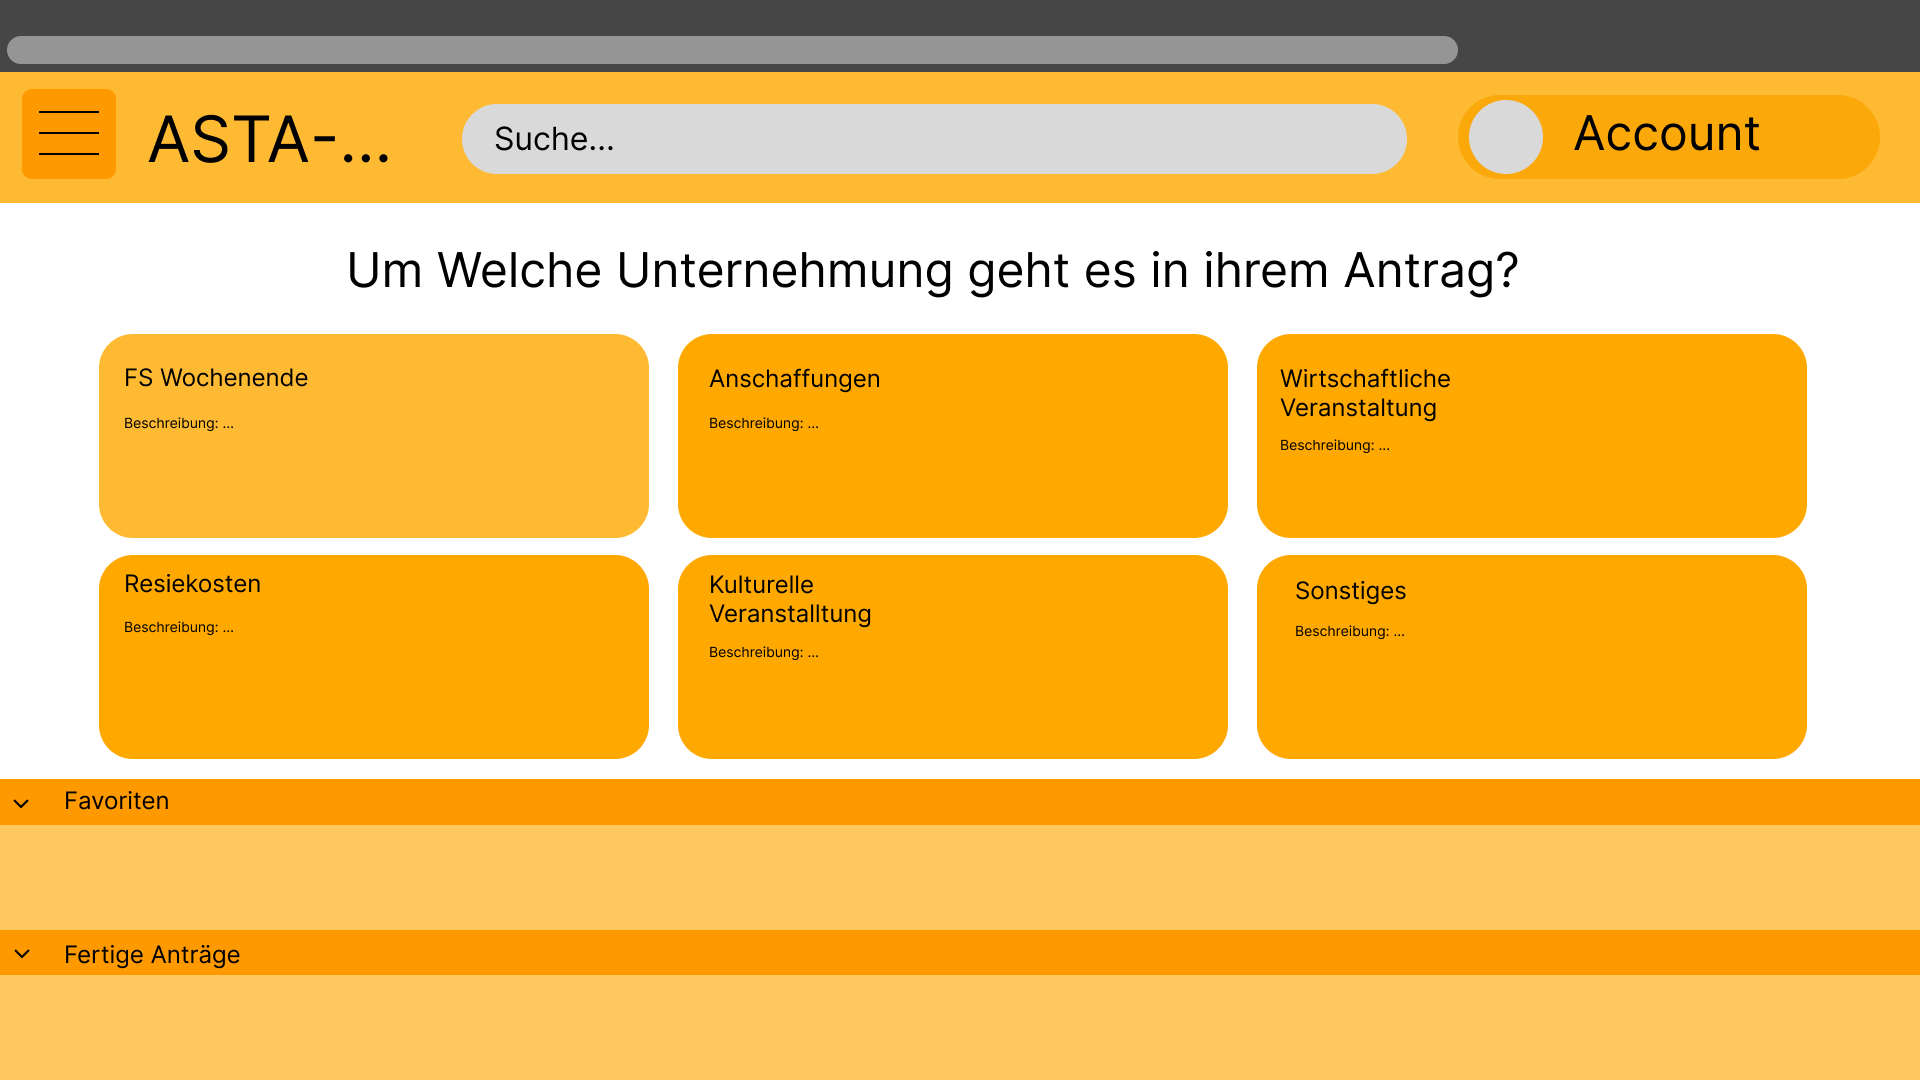
\includegraphics[width=1.0\textwidth]{Antragshelfer}
    \caption{Antragshelfer}\label{Antragshelfer}
\end{figure}
Das Layout des Prototyps lässt sich in drei Bereiche einteilen. Die Kopfzeile, den
Hauptinhalt der Seite sowie die Fußzeile.

In der Kopfzeile befindet sich das AStA-Logo, sowie eine Suchleiste um manuell nach
Anträgen zu suchen. Auch der jeweiligen Nutzeraccount lässt sich über die Schaltfläche
am rechten Rand erreichen. Außerdem befindet sich am linken Rand ein Burger Menü,
welches das Hinzufügen von Funktionalitäten in zukünftigen Projekten erleichtern soll.

Der Hauptinhalt der Seite stellt die Hauptfunktionalitäten unserer Applikation dar und
ist daher in der fertigen Applikation dynamisch generiert. Bei den Prototypen wird dies
durch ein statisches Layout simuliert.

Durch die Fußzeile soll der Nutzer die Möglichkeit erhalten, schnell und einfach auf von
ihm zuvor festgelegten Anträge zugreifen zu können, was eine gute User Experience
gewährleisten soll. Zu erwähnen ist, dass sowohl Kopf- als auch Fußzeile auf jeder Seite
der Applikation identisch sind. Lediglich die Hauptinhalte unterscheiden sich.

Da der Antragshelfer die Hauptfunktionalität unserer Applikation darstellt, fungiert
dieser auch als Landing-Page, also der Seite, welche der Nutzer direkt nach dem Login
sieht, wie in \ref{Antragshelfer} dargestellt. Hier soll der Nutzer durch Klicken mehrerer Buttons die
ihm, von der Applikation gestellten, Fragen beantworten, um so zum richtigen Antrag zu
gelangen. Um dies zu erleichtern, ist jeder Button mit einer Beschreibung versehen, welche genauere Informationen über die Auswahloption liefert.

\begin{figure}[h]
  \centering
    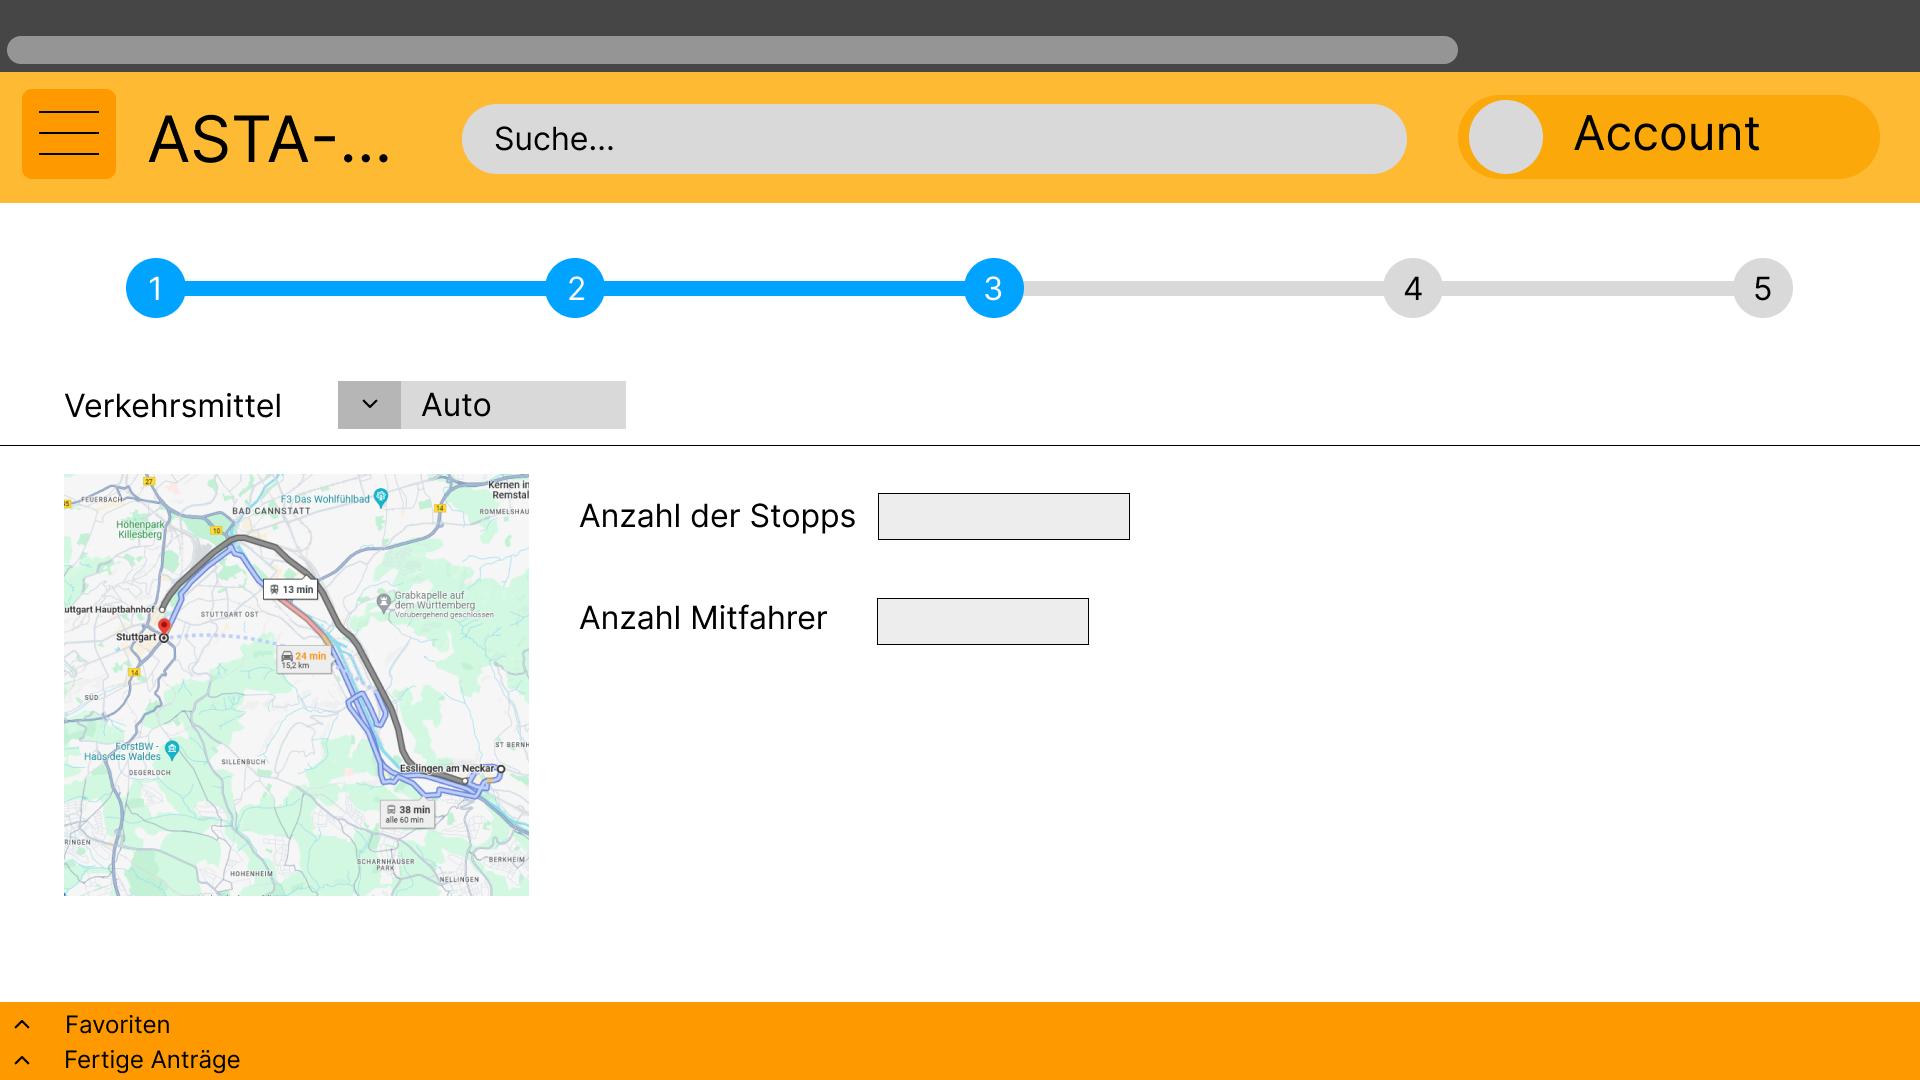
\includegraphics[width=1.0\textwidth]{Reisekostenhelper}
    \caption{Reisekostenhelfer}\label{Reisekostenhelfer}
\end{figure}


Beim Ausfüllen des Antrags hat der Nutzer die Möglichkeit über unterschiedliche Eingabemöglichkeiten, wie Textfelder, Dropdown Menüs oder Checkboxen, die benötigten Informationen einzugeben. Auch die Eingabe über die integrierten APIs ist möglich, wie in \ref{Reisekostenhelfer} am Beispiel eines Reisekosten Antrags zu sehen. Um dem Nutzer einen Überblick über den Fortschritt beim Ausfüllen des Antrags zu ermöglichen, befindet sich am oberen Rand des Hauptinhalts eine Fortschrittsanzeige. So soll der Nutzer darüber informiert werden, wie viele Schritte noch nötig sind, bis der Antrag fertig bearbeitet ist. 



